\section{Counterterms and Non-Analytic Contributions}
\subsection{Review}
We were studying the interacting scalar field theory:
\begin{equation}
    S = -\int d^Dx \frac{1}{2}(\p\phi)^2 + \frac{1}{2}m^2\phi^2 + \frac{1}{3!}\lambda \phi^3
\end{equation}
We found that the 2-point function receives a $O(\lambda^2)$ correction:
\begin{equation}
    \avg{\phi(x)\phi(0)}_C = \avg{\phi(x)\phi(0)}_0 + \frac{i^2}{2}\left.\avg{\phi(x)S_{\text{int}}^2 \phi(0)}_0\right|_{\text{connected diagram}} + O(\lambda^4)
\end{equation}
where we note that there is no $\lambda^3$ correction as the free theory has a $\mathbb{Z}_2$ symmetry. In momentum space:
\begin{equation}
    G_{\text{int}}(p) = G(p) + \delta G(p)_{(A)} + \delta G(p)_{(B)} + \ldots = \frac{-i}{p^2 + m^2- \Pi(p)}
\end{equation}
which in terms of Feynman space Feynman diagrams:

\begin{center}
    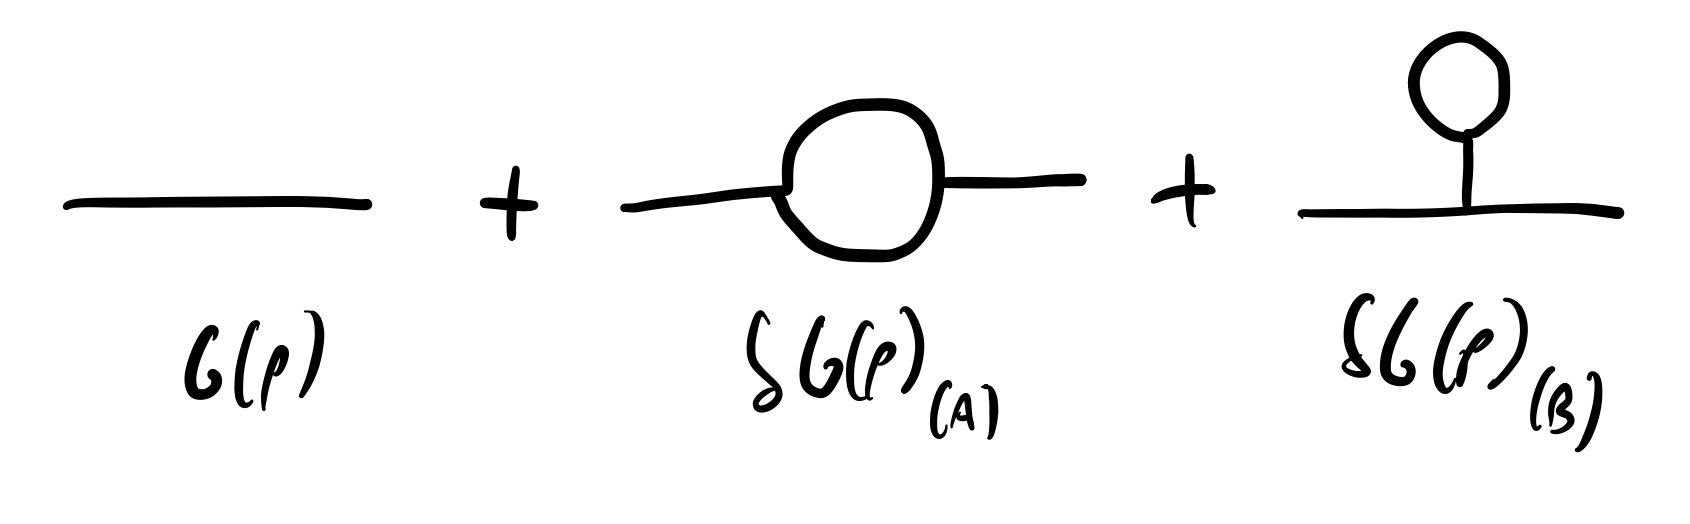
\includegraphics[scale=0.3]{Lectures/Figures/lec13-threediagrams.png}
\end{center}

The self-energy $\Pi(p)$ has two contributions, from the (A) diagram and the (B) diagram. The (A) diagram has contribution (the $(B)$ diagram contribution you study in PS6):
\begin{equation}
    \Pi_{(A)}(p) = \frac{i}{2}\lambda^2\int \frac{d^Dp'}{(2\pi)^D}G(p')G(p - p')
\end{equation}
Note that the (A) diagram gives non-analytic contributions, which is what gives the theory some predictive power. The (B) diagram only has an analytic contribution. Diagramatically, the (A) self-energy looks like the truncated version of the (A) Green's function correction:

\begin{center}
    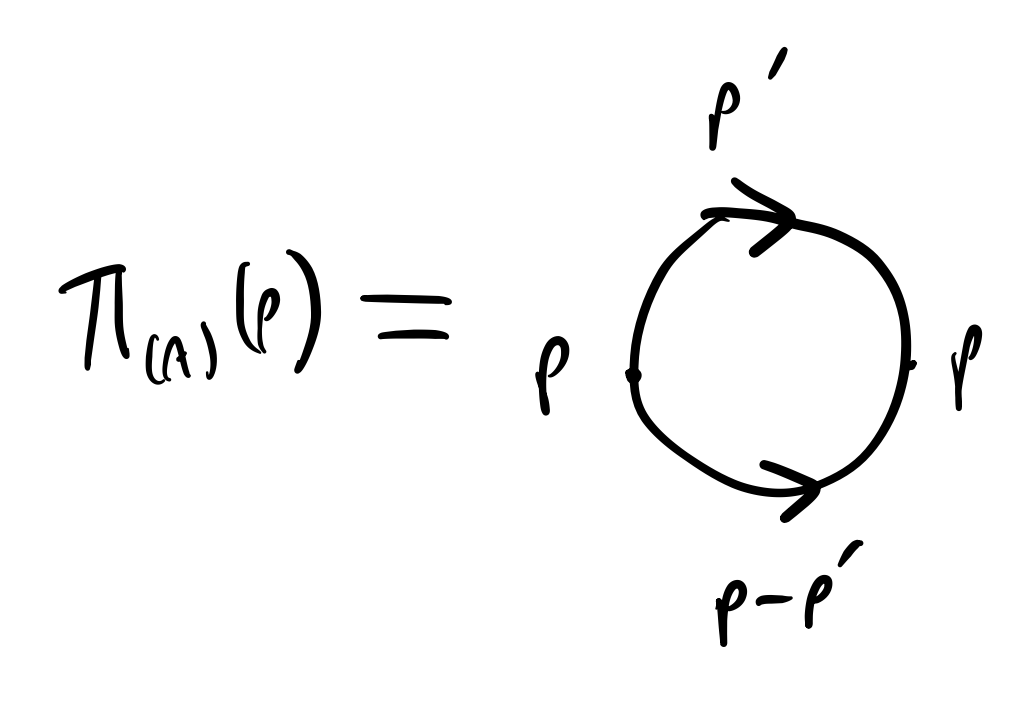
\includegraphics[scale=0.3]{Lectures/Figures/lec13-selfenergy.png}
\end{center}

We took steps towards computing the $\Pi_{(A)}$ integral. We introduced Feynman parameters to bring the two Green's functions over a single denominator, and then Wick rotated to convert the Minkowski product (with negative sign on the $0$th component of momentum) to the standard Euclidean product. Our result was spherically symmetric, and we we were left with:
\begin{equation}
    \Pi_{(A)}(p) = \frac{\lambda^2}{2}\frac{S_{D-1}}{(2\pi)^D}\int_0^1 dx \int_0^\infty dq_E \frac{q_E^{D-1}}{[q_E^2 + \Delta]^2}
\end{equation}
with $\Delta = m^2 +p^2x(1-x)$. This integral converges at $q_E = 0$, but as $q_E \infty$ the integrand goes as $\frac{q_E^{D-1}}{q_E^4} = q_E^{D-5}$ so as long as $D \geq 4$ the integral is UV divergent.

\subsection{Removing analytic divergences - counterterms}
So, we performed this integral with a regulator; a sharp momentum cutoff $\Lambda$. With this cutoff, we found (in $D = 4$):
\begin{equation}
   \int_0^\Lambda dq_E \frac{q_E^{3}}{(q_E^2 + \Delta)^2} = \frac{1}{2}\log \Lambda^2 - \frac{1}{2}\log \Delta(x, p^2) - \frac{1}{2} + O(\frac{1}{\Lambda^2})
\end{equation}
Thus:
\begin{equation}
    \Pi_{(A)}(p) = \frac{\lambda^2}{(4\pi)^2}\int_0^1 dx \frac{1}{2}\log \Lambda^2 - \frac{1}{2} - \frac{1}{2}\Delta(x, p^2) = \frac{\lambda^2}{(4\pi)^2}(\log\Lambda - \frac{1}{2}) - \frac{\lambda^2}{(4\pi)^2}\frac{1}{2}\int_0^1 dx \log\Delta(x, p^2)
\end{equation}
where the first term has no $p$-dependence and the second term has a non-analytic $p$-dependence. The full propagator is:
\begin{equation}
    G_{\text{int}}(p) = \frac{-i^2}{p^2+ m^2 - \Pi(p)}
\end{equation}
So; what we see is that the constant ($p$ independent) piece is just a shift of the mass. If $m$ is the bare mass that I had in the Lagrangian, this does not actually correspond to the pole of the propagator that is measured in the experiment. Further, its a UV divergent correction. But, crucially, this UV divergence can be removed by adding a local counterterm:
\begin{equation}
    \mathcal{L}_{ct} = -\frac{1}{2}\delta m^2 \phi^2
\end{equation}
with:
\begin{equation}
    \delta m^2 = \frac{\lambda^2}{(4\pi)^2}\log \Lambda
\end{equation}
then there is no divergence. So, if we sacrifice the simple relation between experimental parameters (the true mass) and the parameters in the Lagrangian, then we can remove the infinities, here. This tells us that we are not able to predict the mass/poles in this model. But, we can predict other things.

In PS6, you will set $D \geq 6$ and in this case, there are extra UV divergences. In $D = 6$ we see a subleading divergence in $p^2$:
\begin{equation}
    \Pi(p^2) = \lambda^2(c_1\Lambda^2 + c_2p^2\log\Lambda + \ldots)
\end{equation}
Because this divergence is analytic in momentum, we can remove it by adjusting derivative terms. The original Lagrangian had a $(\p\phi)^2$ term, but we can further add a $\frac{\delta Z}{2}(\p \phi)^2$ term to cancel it out. This is a very general approach to QFT, where divergences tell us about what cannot be predicted by the theory.

Perspectives on the UV cutoff; if not a HEP theorist, QFT is just an approximation to the system (an EFT), and in this case the cutoff is just a way of specifying where the EFT breaks down. Another perspective is that interacting QFTs are not defined with just an action; we need an action \emph{and} a regulator. 

\subsection{Renormalization Schemes}
One must choose - for bookkeeping - a ``renormalization scheme''.

For example, in the ``minimal subtraction'' scheme, one adds $\mathcal{L}_{ct}$ with $\delta m^2 = \frac{\lambda^2}{(4\pi)^2}\log \Lambda$. Doing this, the interacting Green's function will be:
\begin{equation}
    G_{\text{int}}(p) = \frac{-i}{p^2 + m_{\text{bare}}^2 + \text{finite}} \implies m_{\text{phys}}^2 = m_{\text{bare}}^2 + \text{finite}
\end{equation}
where the finite correction comes from the loop integral. Another perscription, which is what Srednicki uses, is to insist that the Lagrangian parameter $m_{\text{bare}}^2 = m_{\text{phys}}^2$; so, the counterterm is chosen to remove everything but this, i.e.:
\begin{equation}
    \delta m^2 = \frac{\lambda^2}{(4\pi)^2}\log \Lambda - \text{finite}
\end{equation}
so the pole is at $m_{\text{bare}}^2 = m_{\text{phys}}^2$. We all agree (experimentally) where the pole is, but the Lagrangian parameters may change. 

The bottom line - the relation between bare parameters and the true physical parameters is a subtle one.

\subsection{Non-analyticity and the continuum}
So far, this seems frustrating; we try to compute things in interacting QFTs, and all we learn is that the location of the pole is not something that we can predict. So now, let's talk about the good news, and talk about where interacting QFTs have predictive power. Let us study the non-analytic part of the self-energy:
\begin{equation}
    \Pi(p) = \text{analytic} - \frac{\lambda^2}{(4\pi)^2}\frac{1}{2}\int_0^1 dx \log \Delta(x, p^2), \quad \Delta = m^2 + p^2x(1-x)
\end{equation}
This piece is very interesting. Plugging it into mathematica, we have the result:
\begin{equation}
    \Pi(p) = \text{analytic} - \frac{\lambda^2}{(4\pi)^2}\frac{\text{arctanh}(\sqrt{\frac{p^2}{4m^2 + p^2}})}{\sqrt{\frac{p^2}{4m^2 + p^2}}}
\end{equation}
Where are the singularities of this integral? Let's explore its analytic structure. First, we have a denominator which could diverge. But, in fact this is not a singularity, because we have something of the form $\frac{\text{arctanh}(x)}{x}$, which is not actually singular as $x \to 0$ (due to the arctanh going to $0$ as well; in fact this function is analytic for $\abs{x} \leq 1$). So, $p \to 0$ is not a singularity. We do have singularities coming from the square roots, namely a branch point near $p^2= -4m^2$.

\begin{center}
    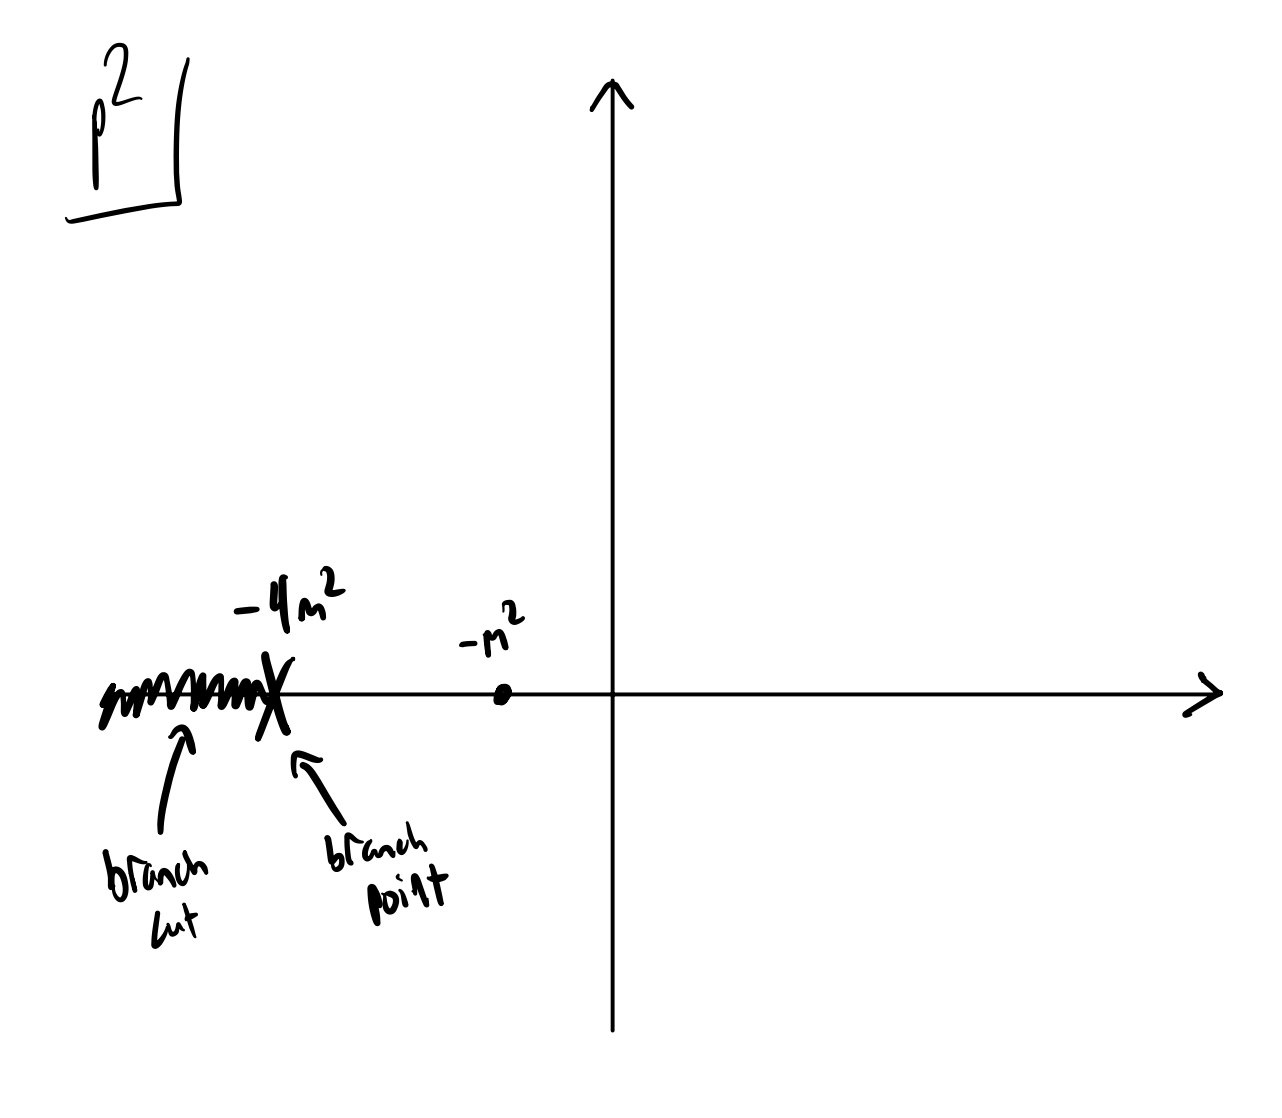
\includegraphics[scale=0.4]{Lectures/Figures/lec13-nonanalytic.png}
\end{center}

These non-analyticities are insensitives to UV divergences/counterterms. They tell us something very physical. Let's see what - it will be more intuitive to see what these are in terms of energy/frequency $p_0$. The non-analyticity is for:
\begin{equation}
    -p_0^2 + \v{p}^2 = p^2 \leq -4m^2 \implies p_0^2 \geq \v{p}^2 + 4m^2 \implies p_0 \geq \sqrt{\v{p}^2 + (2m)^2}
\end{equation}
Plotting this:

\begin{center}
    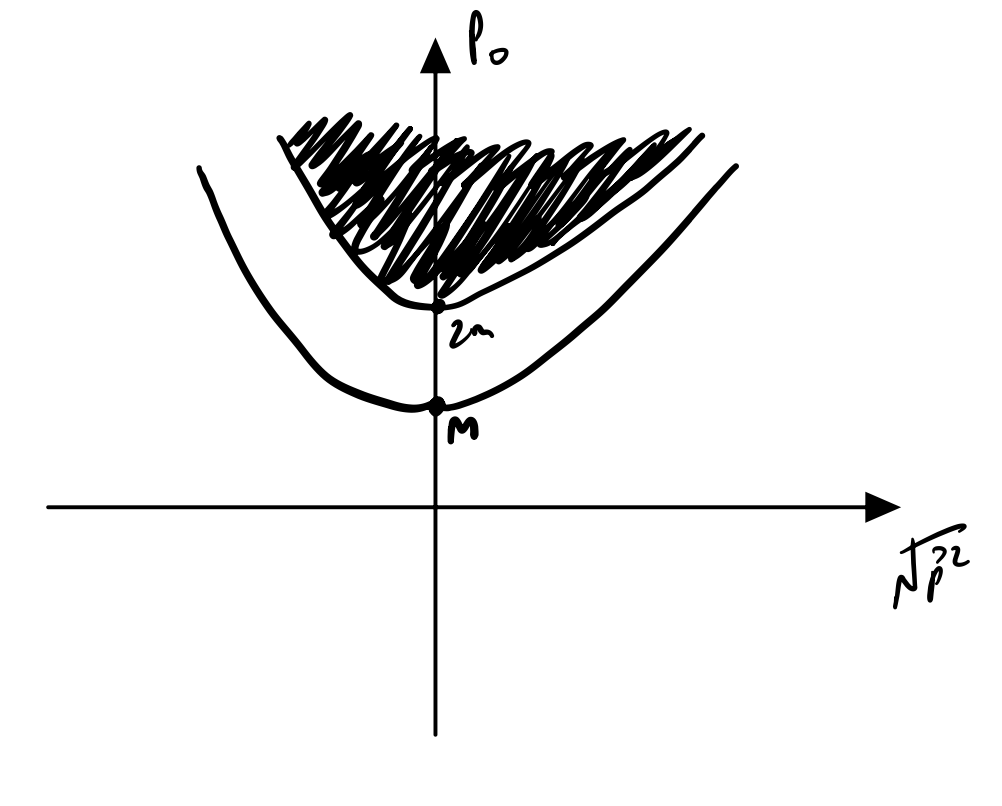
\includegraphics[scale=0.4]{Lectures/Figures/lec13-dispersion.png}
\end{center}

Which looks a lot like our plot in PS1! This is the continuum of two-particle states. They see this because of interactions; in our interacting theory, the particle splits into two particles, and this is what the experimentalist sees.

In these regions, $\text{Re}G \neq 0$. In the free theory:
% The Feynman's green functions are almost purely imaginary; but there is a small contribution from the $-i\e$ in the denominator. 
\begin{equation}
    \text{Re}G(p) = \text{Im}\frac{1}{p^2 + m^2 - i\e}
\end{equation}
Then using that $\lim_{\e\to 0}\frac{1}{x - i\e} = \text{(principal value)}\frac{1}{x} + i\pi\delta(x)$, we have:
\begin{equation}
    \text{Re}G(p) = \pi\delta(p^2 + m^2)
\end{equation}
i.e. in the free theory the Green's function only fires on-shell. In the interacting theory, $\text{Re} G \neq 0$ (and $O(\lambda^2)$) for any $\abs{p_0} \geq \sqrt{\v{p}^2 + (2m)^2}$.

The experimentalist knows of a particle-splitting interaction in the theory, and expects to see the two-particle continuum. In the $\lambda \phi^4$ theory, we instead have a (non-analytic) diagram of the form:

\begin{center}
    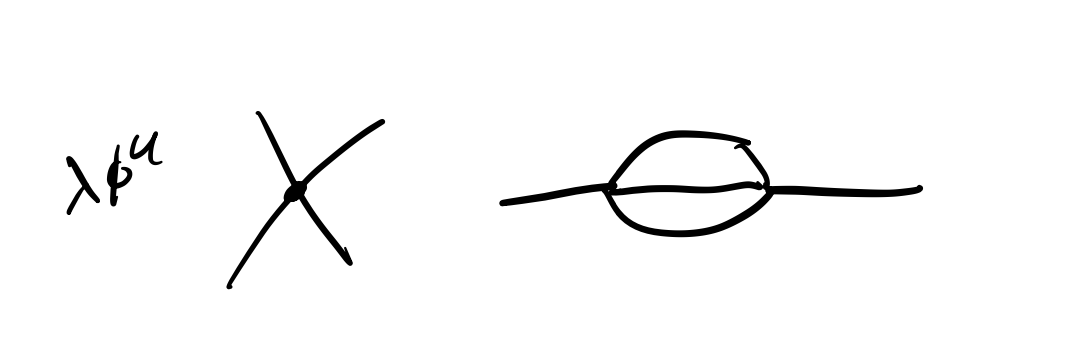
\includegraphics[scale=0.3]{Lectures/Figures/lec13-phi4.png}
\end{center}

where now the particle splits into three particles (the diagram on the right corresponds to the momentum space diagram), so the experimentalist would see a there-particle continuum starting at $3m$.

\subsection{Comments}
\begin{enumerate}
    \item Why have we written $G(p) = \frac{-i}{p^2 + m^2 - \Pi(p)}$ if $\Pi(p) = O(\lambda^2) + \ldots$? We do not know all $O(\lambda^4)$ diagrams. We can draw them:
    \begin{center}
        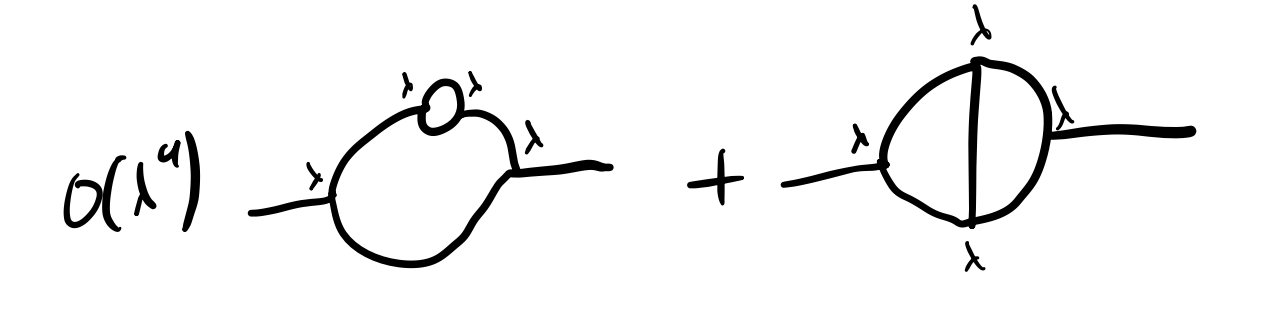
\includegraphics[scale=0.3]{Lectures/Figures/lec13-lambda4.png}
    \end{center}
    but we did not include them. Why? The answer is that often, we are interested in $G_{\text{int}}(p)$ near its pole, where it is largest, i.e. near $p^2 \approx -m^2$. In this regime, the diagrams involving the largest amount of bare propagators, i.e. the largest number of $G(p^2)$s, give the largest contribution. Phrased another way, we are computing small corrections to things (we are working in perturbation theory). If there is a small correction and/or branch cut to the location of the pole, there is a huge correction to the Green's function. Compare the one-loop diagrams (and geometric series of them) with the other $O(\lambda^4)$ diagrams we drew above; they have less factors of $G(p^2)$ and thus contribute less. Having already computed the one-loop diagram and packaging it in $\Pi(p)$ (and hence the correction to $G(p)$ as a geometric series), we have already found the largest contribution.
    \begin{center}
        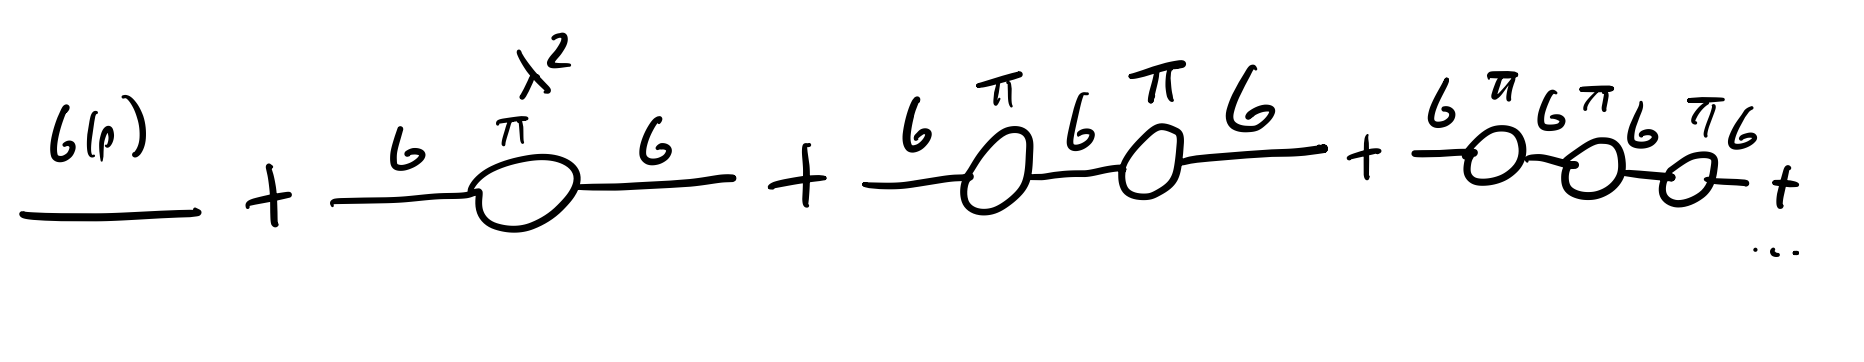
\includegraphics[scale=0.3]{Lectures/Figures/lec13-geomseries.png}
    \end{center}

    Another, related comment; $\Pi(p)$ is a good way to repackage perturbation theory as a whole.  To this end, we are really considering the Taylor series expansion of diagrams that cannot be separated into two with a cut of a single line, also  are know as ``1PI'', or 1-particle irreducible diagrams. Another way to describe them is that there are no intermediate single-particle states. Going to higher order:
    \begin{equation}
        G(p) = \frac{-i}{p^2 + m^2 - \Pi(p)}
    \end{equation}
    already resums the geometric series for any building block. At higher orders this building block contains more complicated objects (more 1PI diagrams exist). But, the general fact is that the Green's function contains all connected diagrams, but they are organized as geometric series in the 1PI diagrams:
    \begin{center}
        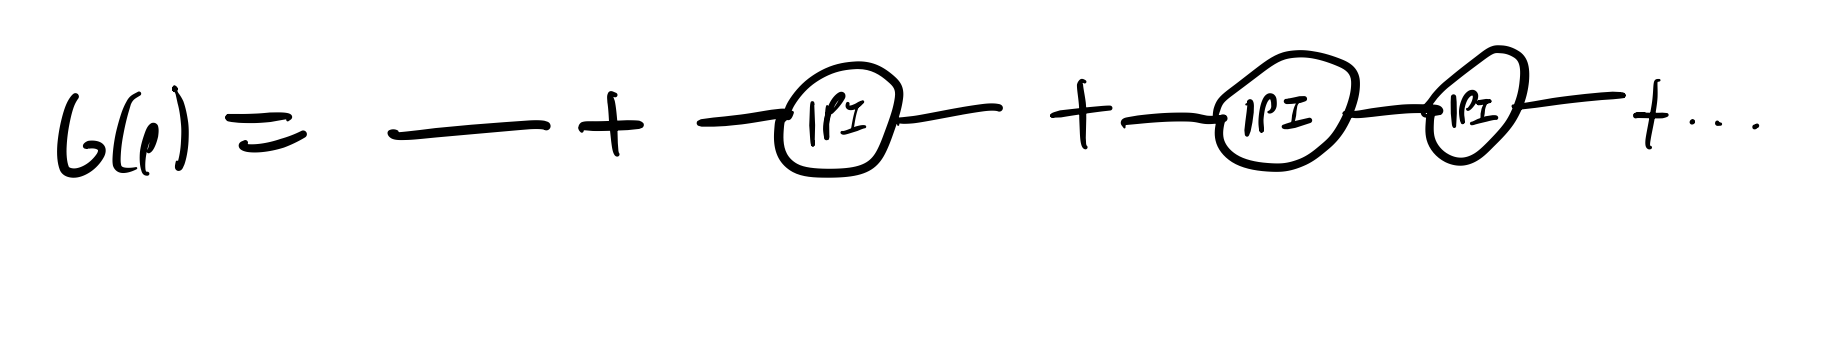
\includegraphics[scale=0.3]{Lectures/Figures/lec13-1PIgeomseries.png}
    \end{center}
    
    Thus, we can equate $\Pi(p)$ with all 1PI diagrams. The 1PI diagrams to $\lambda^4$ in perturbation theory look like:
    \begin{center}
        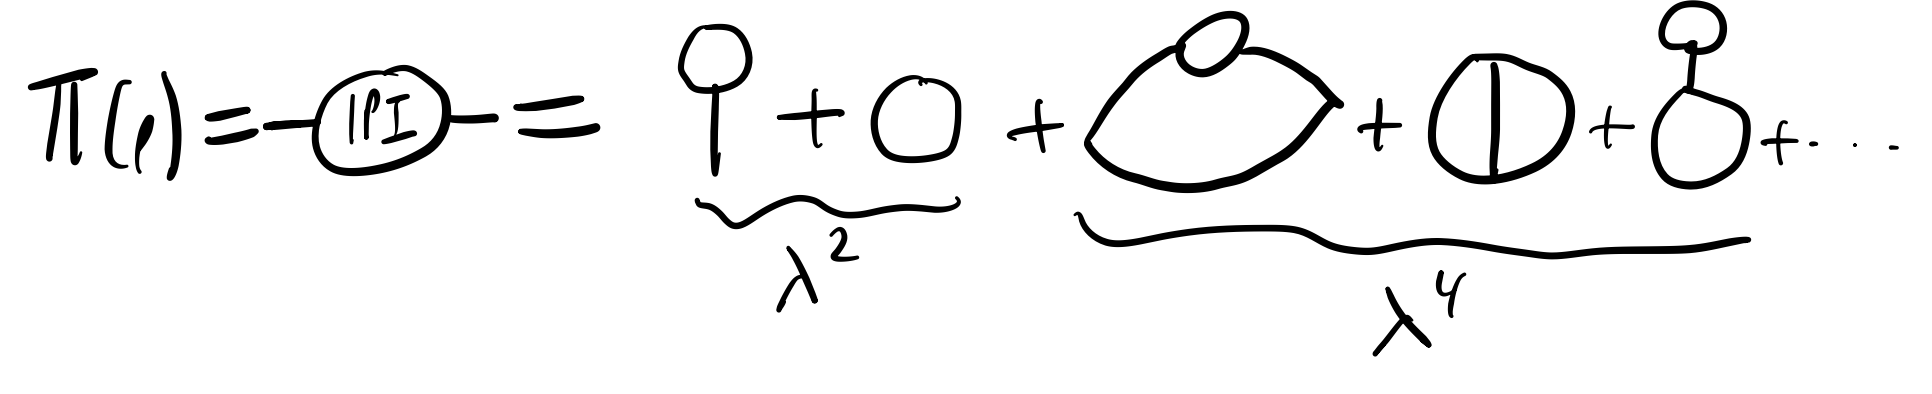
\includegraphics[scale=0.3]{Lectures/Figures/lec13-1PIlambda4.png}
    \end{center}

    \item A second small comment. Physical quantities do \emph{not} depend on the regulator. For the location of the pole/$m_{\text{phys}}^2$, this is a tautological statement, because we did not predict anything. But the location of the branch point at $4m_{\text{phys}}^2$, and the value of the Green's function along the branch cut is something that \emph{cannot} be modified by the choice of the regulator. The UV divergences are helpful in the sense that they tell us where we have predictive power, and where we do not.
    
    \item We are doing perturbation theory in $\lambda$. But of course $\lambda$ is a dimensionful quantity, so saying it is ``small'' does not make much sense on its own. What is the small dimensionless parameter that is giving us control over the expansion? $[\lambda] = \frac{6-D}{2}$, or $\lambda \sim E^{\frac{6-D}{2}}$. In fact, the dimensionless number depends on the energy scale; for example $\frac{\lambda}{p^{\frac{6-D}{2}}}$. For PT to work/be controlled, we need the above dimensionless quantity to be small. More specifically, if $[\lambda] > 0$ (as is the case for $D < 6$), we require the interaction to be large to have control. 
    Interactions are \emph{relevant}, it has a large effect at low energies. Perturbation theory works at high energy in this case. Conversely, if $[\lambda] < 0$ ($D > 6$), then interactions are \emph{irrelevant}, i.e. it has a small effect at low energies. Thus perturbation theory works at $p \ll \lambda^{\#}$. This is the regime of EFT. What if $[\lambda] = 0$, i.e. precisely at $D = 6$? Then, we compare $\lambda$ to $\log(p)$, and we have $G(p) = \frac{1}{p^2}(1 + \lambda^2 \log(p))$. In this case, PT breaks down both at high and low energies. Unfortuantely, it is the case that most couplings in the universe (in the standard model) are dimensionless. What ends up saving us is the renormalization group, which we discuss next day.
\end{enumerate}